\section{Sự đồng biến, nghịch biến của hàm số}
\subsection{Đề 1}
\Opensolutionfile{ans}[ans/ans-2-B1-De1-LC]
\caulc
\begin{ex}%[Câu 1]%[2D1H1-1]
	Cho hàm số $y=\dfrac{8-5x}{-4x-9}$. Khẳng định nào sau đây là \textbf{sai}?
	\choice
	{Hàm số đồng biến trên khoảng $\left(-\infty;-\dfrac{37}{4}\right)$}
	{Hàm số đồng biến trên khoảng $\left(-\infty;-\dfrac{9}{4}\right)$}
	{Hàm số đồng biến trên khoảng $\left(-\dfrac{9}{4};+\infty\right)$}
	{\True Hàm số nghịch biến trên khoảng $\left(-\infty;-\dfrac{37}{4}\right)$}
	\loigiai{
		Tập xác định $\mathscr{D}=\mathbb{R}\backslash\left\{-\dfrac{9}{4}\right\}$.\\
		$y'=\dfrac{-5\cdot(-9)-8\cdot(-4)}{\left(-4x-9\right)^{2}}=\dfrac{77}{\left(-4x-9\right)^{2}}>0,\forall x \in \mathscr{D}$.\\
		Do đó, hàm số đồng biến trên mỗi khoảng $\left(-\infty;-\dfrac{9}{4}\right)$ và $\left(-\dfrac{9}{4};+\infty\right)$.
	}
\end{ex}

\begin{ex}%[Câu 2]%[2D1N1-2]
	Cho hàm số có bảng biến thiên như sau
	\begin{center}
		\begin{tikzpicture}
			\tkzTabInit[nocadre=false, lgt=1, espcl=2] 
			{$x$ /1,$y'$ /0.7,$y$ /1.7}
			{$-\infty$,$\dfrac{-4}{3}$,$\dfrac{1}{2}$,$+\infty$}
			\tkzTabLine{,+,0,-,0,+,} 
			\tkzTabVar{-/$-\infty$ ,+/ $\dfrac{218}{27}$, -/ $\dfrac{-17}{4}$ /, +/$+\infty$ /} 
		\end{tikzpicture}
	\end{center}
	Khẳng định nào sau đây là \textbf{đúng}?
	\choice
	{Hàm số nghịch biến trên khoảng $\left(-\infty;-\dfrac{4}{3}\right)$}
	{Hàm số đồng biến trên khoảng $\left(-\dfrac{4}{3};\dfrac{1}{2}\right)$}
	{Hàm số nghịch biến trên khoảng $\left(\dfrac{7}{2};+\infty\right)$}
	{\True Hàm số đồng biến trên khoảng $\left(-\infty;-\dfrac{7}{3}\right)$}
	\loigiai{
		Dựa vào bảng biến thiên ta thấy, hàm số đồng biến trên mỗi khoảng $\left(-\infty;-\dfrac{4}{3}\right)$ và $\left(\dfrac{1}{2};+\infty\right)$.\\
		Hàm số nghịch biến trên $\left(-\dfrac{4}{3};\dfrac{1}{2}\right)$.
	}
\end{ex}

\begin{ex}%[Câu 3]%[2D1N1-2]
	\immini{Cho hàm số có đồ thị như hình bên. Khẳng định nào sau đây là \textbf{đúng}?
		\choice
		{Hàm số nghịch biến trên khoảng $(-\infty;1)$}
		{Hàm số nghịch biến trên khoảng $(-\infty;0)$}
		{Hàm số nghịch biến trên khoảng $\left(\dfrac{7}{3};+\infty\right)$}
		{\True Hàm số đồng biến trên khoảng $(-\infty;1)$}
	}{
		\begin{tikzpicture}[line cap=round,>=stealth,scale=0.4]
			\tikzset{every node/.style={scale=0.5}}
			\draw[->] (-3.333,0)--(6.667,0) node[below left] {$x$};
			\draw[->] (0,-3.593)--(0,10.407) node[below left] {$y$};
			\draw (0,0) node [below left] {$O$};
			\draw[dashed](1,0) node[below] {$1$}--(1,4)(2.333,0) node[below] {$\dfrac{7}{3}$}--(2.333,2.815);
			\begin{scope}
				\clip (-3.333,-3.493) rectangle (6.667,10.307);
				\draw[samples=100,domain=-3.233:6.567,smooth,variable=\x] plot (\x,{1*((\x)^3)-5*((\x)^2)+7*(\x)+1});
			\end{scope}
		\end{tikzpicture}
	}
	\loigiai{
		Dựa vào đồ thị ta thấy, hàm số đồng biến trên mỗi khoảng $(-\infty;1)$ và $\left(\dfrac{7}{3};+\infty\right)$.\\
		Hàm số nghịch biến trên $\left(1;\dfrac{7}{3}\right)$.
	}
\end{ex}

\begin{ex}%[Câu 4]%[2D1H1-3]
	Tìm tất cả các giá trị thực của tham số $m$ để hàm số $y=-\dfrac{1}{3}x^3-mx^2+(2m-3)x-m+2$ nghịch biến trên  $\mathbb{R}$.
	\choice
	{$m\le -3$, $m\ge 1$}
	{$-3<m<1$}
	{\True  $-3\le m\le 1$}
	{$m\le 1$}
	\loigiai{
		Ta có $y'=-x^2-2mx+(2m-3)$.\\
		Hàm số nghịch biến trên $\mathbb{R}$ khi
		\begin{align*}
			&~ y'\le 0 \\
			\Leftrightarrow &~ \heva{a&=-1<0\\ \Delta'& \le 0} \\
			\Leftrightarrow &~ m^2+2m-3\le 0 \\
			\Leftrightarrow &~-3\le m \le 1.
		\end{align*}
	}
\end{ex}

\begin{ex}%[Câu 5]%[2D1V1-3]
	Cho hàm số $y=-x^3-mx^2+(4m+9)x+5$, với $m$ là tham số thực. Có bao nhiêu giá trị nguyên của $m$ để hàm số nghịch biến trên $(-\infty;+\infty)$?
	\choice
	{$5$}
	{ $6$}
	{ \True $7$ }
	{$4$}
	\loigiai{ 
		Hàm số $y=-x^3-mx^2+(4m+9)x+5$ là hàm bậc 3 có hệ số $a=-1<0$ nên điều kiện cần và đủ để $y=-x^3-mx^2+(4m+9)x+5$ nghịch biến trên $(-\infty;+\infty)$ là
		\begin{align*}
			&~ y'=-3x^2-2mx+4m+9\le 0, \forall x\in\mathbb{R} \\
			\Leftrightarrow &~ \Delta'=m^2+12m+27\le 0 \\
			\Leftrightarrow &~ -9\le m\le -3 \\
			\Rightarrow &~ m\in\{-9,-8,-7,-6,-5,-4,-3\}.
		\end{align*}
	}
\end{ex}

\begin{ex}%[Câu 6]%[2D1H2-1]
	Cho hàm số $y=7x^3+9x^2-3x-4$. Khẳng định nào sau đây là \textbf{sai}?
	\choice
	{Giá trị cực đại $y=1$}
	{Hàm số đạt cực tiểu tại $x=\dfrac{1}{7}$}
	{\True Giá trị cực tiểu $y=\dfrac{1}{7}$}
	{Hàm số đạt cực đại tại $x=-1$}
	\loigiai{
		Tập xác định $\mathbb{R}$.\\
		$y'=21x^2+18x-3$.\\
		$y'=0 \Leftrightarrow x=-1 \text{ hoặc } x=\dfrac{1}{7}$.\\
		Do đó, hàm số đạt cực đại tại $x=-1, y_{\text{CĐ}}=1$.\\
		Hàm số đạt cực tiểu tại $x=\dfrac{1}{7}, y_{\text{CT}}=- \dfrac{207}{49}$.
	}
\end{ex}

\begin{ex}%[Câu 7]%[2D1N2-2]
	Cho hàm số $y=f(x)$ xác định trên $\mathbb{R}$ và có bảng biến thiên như hình vẽ sau
	\begin{center}
	\begin{tikzpicture}
		\tkzTabInit[nocadre=false, lgt=1, espcl=2] 
		{$x$ /0.6,$y'$ /0.7,$y$ /1.7}
		{$-\infty$,$10$,$12$,$+\infty$}
		\tkzTabLine{,+,0,-,0,+,} 
		\tkzTabVar{-/$-\infty$ ,+/$-3$, -/ $3$ /, +/$-\infty$ /} 
	\end{tikzpicture}
	\end{center}
	Hàm số $y=f(x)$ đạt cực đại tại
	\choice
	{ \True $x=10$}
	{ $x=8$}
	{ $x=12$}
	{ $x=17$}
	\loigiai{
	Dựa vào bảng biến thiên ta thấy hàm số đạt cực đại tại $x=10$.
	}
\end{ex}

\begin{ex}%[Câu 8]%[2D1N2-2]
	\immini{Cho hàm số có đồ thị như hình bên. 
		Khẳng định nào \textbf{sai}?
		\choice
		{Hàm số có một cực tiểu tại $x=\dfrac{3}{4}$ và đạt cực đại tại $x=0$}
		{Giá trị cực đại $y=-1$ và giá trị cực tiểu $y=-\dfrac{113}{32}$}
		{Hàm số có một cực tiểu tại $x=-\dfrac{3}{4}$}
		{\True Hàm số có một cực đại tại $x=-\dfrac{3}{4}$}
	}{
		\begin{tikzpicture}[line cap=round,>=stealth,scale=0.9]
			\tikzset{every node/.style={scale=0.8}}
			\draw[->] (-1.75,0)--(1.75,0) node[below left] {$x$};
			\draw[->] (0,-4.531)--(0,1) node[below left] {$y$};
			\draw (0,0) node [below left] {$O$};
			\draw[dashed,thin](-0.75,0) node[above] {$-\dfrac{3}{4}$}--(-0.75,-3.531)--(0.75,-3.531)--(0.75,0) node[above] {$\dfrac{3}{4}$};
			\path(0,-3.531) node[below left] {$-\dfrac{113}{32}$} (0,-1) node[above right]{$-1$};
			\begin{scope}
				\clip (-1.75,-4.431) rectangle (1.75,0.9);
				\draw[samples=200,domain=-1.65:1.65,smooth,variable=\x] plot (\x,{8*((\x)^4)-9*((\x)^2)-1});
			\end{scope}
		\end{tikzpicture}
	}
	\loigiai{
		Dựa vào đồ thị ta thấy, hàm số đạt cực đại tại $x=0, y_{\text{CĐ}}=-1$.\\
		Hàm số đạt cực tiểu tại $x=-\dfrac{3}{4}$ và $x=\dfrac{3}{4}$, $y_{\text{CT}}=-\dfrac{113}{32}$.
	}
\end{ex}

\begin{ex}%[Câu 9]%[2D1H2-3]
	Cho hàm số $y = 8x^3 -6mx^2 + 9mx + 6m$ ($m$ là tham số thực). Giá trị của $m$ để hàm số đạt cực tiểu tại $x=-6$ thuộc khoảng nào sau đây?
	\choice
	{$\left(-\infty;-\dfrac{35}{3}\right)$}
	{$\left(-\infty;-\dfrac{47}{3}\right)$}
	{$\left(-\dfrac{23}{3}; +\infty\right)$}
	{\True $\varnothing$}
	\loigiai{
		Hàm số xác định với mọi $x \in \mathbb{R}$.\\
		Ta có $y'=24x^2 -12mx + 9m$.\\
		Hàm số đạt cực tiểu tại $x=-6 \Rightarrow y'(-6) = 0 \Leftrightarrow 81m+864 = 0 \Leftrightarrow m=-\dfrac{32}{3}$.\\
		Thử lại:\\
		Với $m = -\dfrac{32}{3}$, ta có: $y'(-6) = 0$ và $y''(-6) = -160 < 0$.\\
		$\Rightarrow x=-6$ là điểm cực đại của hàm số.\\
		Vậy không có giá trị nào của $m$ thoả bài toán.
	}
\end{ex}

\begin{ex}%[Câu 10]%[2D1H2-4]
	Tìm tất cả các giá trị thực của $m$ để hàm số $y=x^3-3x^2+(m+1)x+2$ có hai điểm cực trị.
	\choice{\True $m<2$}
	{$m\le 2$}
	{$m>2$}
	{$m<-4$}
	\loigiai{
		$y'=3x^2-6x+m+1$, $\Delta'=6-3m$.\\
		Để hàm số có hai điểm cực trị thì $y'=0$ phải có hai nghiệm phân biệt tức là\\
		$\Delta'>0\Leftrightarrow m<2$.
	}
\end{ex}

\begin{ex}%[Câu 11]%[2D1V2-4]
	Cho hàm số $y = x^3 -2mx^2 + \left(- \dfrac{4}{3}m^2 -40m -144\right)x -5$ ($m$ là tham số thực). Tìm tất cả các giá trị của $m$ để hàm số có cực trị?
	\choice
	{$-11 < m < -6$}
	{$m < -9$ hoặc $m > -4$}
	{$-14 < m < -6$}
	{\True $m < -9$ hoặc $m > -6$}
	\loigiai{
		Hàm số xác định với mọi $x \in \mathbb{R}$.\\
		Ta có $y'=3x^2 -4mx - \dfrac{4}{3}m^2 -40m -144$.\\
		Hàm số có cực trị khi phương trình $3x^2 -4mx - \dfrac{4}{3}m^2 -40m -144=0$ có 2 nghiệm phân biệt\\
		$\Leftrightarrow \Delta' > 0 \Leftrightarrow m^2 + 15m + 54 > 0 \Leftrightarrow m < -9$ hoặc $m > -6$.
	}
\end{ex}

\begin{ex}%[Câu 12]%[2D1V2-5]
	Cho hàm số $y=(m+1)x^4-mx^2+3$. Tìm tất cả các giá trị thực của tham số $m$ để hàm số có ba điểm cực trị.
	\choice
	{$m\in (-\infty;-1)\cup [0;+\infty)$}
	{$m\in (-1;0)$}
	{$m\in (-\infty;-1]\cup [0;+\infty)$}
	{\True $m\in (-\infty;-1)\cup (0;+\infty)$}
	\loigiai{
		$y^\prime= 4(m+1)x^3-2mx=2x[2(m+1)x^2-m]$\\
		$y^\prime =0\Leftrightarrow \hoac{&x=0\\&2(m+1)x^2-m=0\,\,(*)} $\\
		Hàm số có ba điểm cực trị khi phương trình $(*)$ có hai nghiệm phân biệt khác $0$\\$\Leftrightarrow \dfrac{m}{m+1}>0\Leftrightarrow \hoac{&m<-1\\&m>0.} $
	}
\end{ex}
\Closesolutionfile{ans}
\indapan{6}{ans/ans-2-B1-De1-LC}
%-------------------------------------------
\Opensolutionfile{ans}[ans/ans-2-B1-De1-DS]
\cauds
\begin{ex}%[Câu 13]%[2D1H1-1]
	Cho hàm số $y=f(x)=x^3-3x^2-1$. Các mệnh đề sau đúng hay sai?
	\choiceTF
	{Hàm số đã cho nghịch biến trên $\mathbb{R}$}
	{\True Hàm số đã cho đồng biến trên $(3;+\infty)$}
	{\True Hàm số đã cho nghịch biến trên $(1;2)$}
	{\True Hàm số $g(x)=f(x)+2$ đồng biến trên $(-\infty;0)$}
	\loigiai{
		$y'=3x^2-6x$. Giải $y'=0$ ta được $x=0$, $x=2$.
		\begin{center}
			\begin{tikzpicture}
				\tkzTabInit[nocadre=false, lgt=1, espcl=2] 
				{$x$ /0.7,$y'$ /0.7,$y$ /1.7}
				{$-\infty$,$0$,$2$,$+\infty$}
				\tkzTabLine{,+,0,-,0,+}  
				\tkzTabVar{-/$-\infty$ ,+/ $-3$, -/ $-5$ /, +/$+\infty$ /}  
			\end{tikzpicture}
		\end{center}
		\begin{itemchoice} 
			\itemch Hàm số không nghịch biến trên $\mathbb{R}$.
			\itemch Hàm số đã cho đồng biến trên $(3;+\infty)$.
			\itemch Hàm số đã cho nghịch biến trên $(1;2)$.
			\itemch Hàm số $g(x)=f(x)+2$ đồng biến trên $(-\infty;0)$.
		\end{itemchoice}
	}
\end{ex}

\begin{ex}%[Câu 14]%[2D1V1-2]
	\immini
	{
	Cho hàm số $y=f(x)$ có đồ thì như hình vẽ bên. Các mệnh đề sau đúng hay sai?
	\choiceTF
	{\True Hàm số đã cho nghịch biến trên khoảng $(-2,0)$}
	{Hàm số đã cho đồng biến trên khoảng $(-3;1)$}
	{\True Hàm số đã cho đồng biến trên khoảng $(2;+\infty)$}
	{Hàm số $f=|f(x)|$ nghịch biến trên khoảng $(-2,0)$}
	}{
	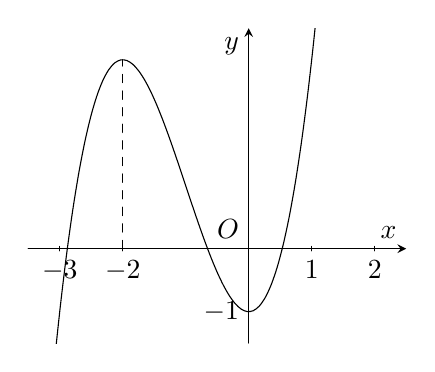
\begin{tikzpicture}[line cap=round,>=stealth,scale=0.8]
		%		\tikzset{every node/.style={scale=0.8}}
		\draw[->] (-3.5,0)--(2.5,0) node[above left] {$x$};
		\draw[->] (0,-1.5)--(0,3.5) node[below left] {$y$};
		\draw (0,0) node [above left] {$O$};
		\draw[dashed,thin](-2,0)--(-2,3) (0,-1) node[left] {$-1$};
		\foreach \x/\nx in {-3/-3, -2/ -2,1/1,2/2}
		\draw[thin] (\x,1pt)--(\x,-1pt) node [below] {$\nx$};
		\begin{scope}
			\clip (-3.5,-1.5) rectangle (2,3.5);
			\draw[samples=100,domain=-4.9:4.567,smooth,variable=\x] plot (\x,{1*((\x)^3)+3*((\x)^2)-1});
		\end{scope}
	\end{tikzpicture}
	}
	\loigiai{
		\begin{itemchoice}
			\itemch Dựa vào đồ thị hàm số ta thấy hàm số nghịch biến trên khoảng $(-2,0)$.
			\itemch Dựa vào đồ thị hàm số ta thấy trên khoảng $(-3;1)$ hàm số đồng biến và nghịch biến.
			\itemch Dựa vào đồ thị hàm số ta thấy hàm số đồng biến trên $(-\infty;-2)$ và $(0;+\infty)$ nên hàm số đồng biến trên khoảng $(2;+\infty)$.
			\itemch Hàm số $y=|f(x)|$ có đồ thị như hình bên dưới. Ta nhận thấy trên khoảng $(2;+\infty)$ hàm số nghịch biến và đồng biến. \\
			\begin{center}
				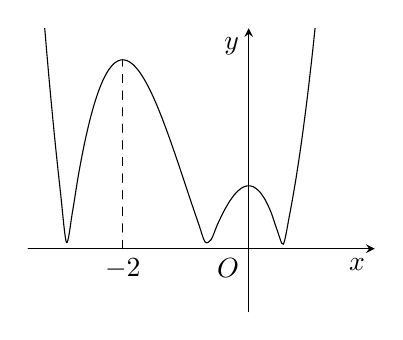
\begin{tikzpicture}[line cap=round,>=stealth,scale=0.8]
					%		\tikzset{every node/.style={scale=0.8}}
					\draw[->] (-3.5,0)--(2,0) node[below left] {$x$};
					\draw[->] (0,-1)--(0,3.5) node[below left] {$y$};
					\draw (0,0) node [below left] {$O$};
					\draw[dashed,thin](-2,0) node[below] {$-2$}--(-2,3);
					\begin{scope}
						\clip (-3.5,-1) rectangle (2,3.5);
						\draw[samples=100,domain=-4.9:4.567,smooth,variable=\x] plot (\x,{abs(1*((\x)^3)+3*((\x)^2)-1)});
					\end{scope}
				\end{tikzpicture}
			\end{center}
		\end{itemchoice}
	}
\end{ex}

\begin{ex}%[Câu 15]%[2D1H2-1]
	Cho hàm số $y=f(x)=x^4-2x^2-3$. Các mệnh đề sau đúng hay sai?
	\choiceTF
	{\True Hàm số đã cho đạt cực đại tại $x=0$}
	{Hàm số đã cho đạt cực tiểu tại $x=-3$}
	{Hàm số đã cho có giá trị cực đại và cực tiểu lần lượt là $-4,-3$}
	{Đồ thị hàm số $g(x)=f(x)+3$ có điểm cực đại là $(0;0)$ }
	\loigiai{
		Ta có $y'=4x^3-4x$. Giải $y'=0$ ta được $x=-1$, $x=0$, $x=1$.\\
		Bảng biến thiên
		\begin{center}
			\begin{tikzpicture}
				\tkzTabInit[nocadre=false, lgt=1, espcl=2] 
				{$x$ /0.7,$y'$ /0.7,$y$ /1.7}
				{$-\infty$,$-1$,$0$,$1$,$+\infty$}
				\tkzTabLine{,-,0,+,0,-,0,+,} 
				\tkzTabVar{+/$-\infty$ ,-/ $-9$, +/ $-3$ /, -/$1$, +/$+\infty$} 
			\end{tikzpicture}
		\end{center}
		\begin{itemchoice}
			\itemch Dựa vào bảng biến thiên ta thấy hàm số đạt cực đại tại $x=0$
			\itemch Dựa vào bảng biến thiên ta thấy hàm số đạt cực tiểu tại $x=-3$
			\itemch Dựa vào bảng biến thiên ta thấy hàm số giá trị cực đại và cực tiểu lần lượt là $-4,-3$
			\itemch Dựa vào bảng biến thiên ta thấy hàm số $g(x)=f(x)+3$ có điểm cực đại là $(0;0)$
		\end{itemchoice}
	}
\end{ex}

\begin{ex}%[Câu 16]%[2D1V2-2]
	\immini{
	Cho hàm số $y=f(x)$ có đồ thị như hình vẽ bên dưới. 
	\choiceTF
	{Hàm số đã cho chỉ có 2 cực trị}
	{Hàm số đã cho có giá trị cực tiểu $x=-2$}
	{\True Hàm số đã cho có giá trị cực đại $y=-1$}
	{\True Đồ thị hàm số $y=|f(x)|$ có điểm cực đại là $(0,2)$}	
	}{
	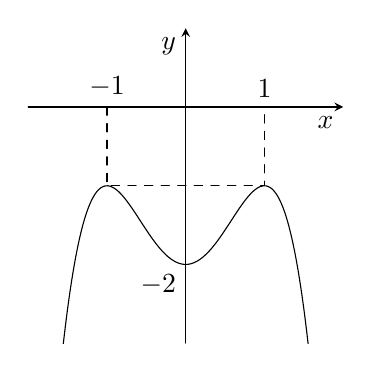
\begin{tikzpicture}[line cap=round,>=stealth,scale=1]
		%		\tikzset{every node/.style={scale=0.8}}
		\draw[->] (-2,0)--(2,0) node[below left] {$x$};
		\draw[->] (0,-3)--(0,1) node[below left] {$y$};
%		\draw (0,0) node [below left] {$O$};
		\draw[dashed,thin](-1,0) node[above] {$-1$}--(-1,-1)--(1,-1)--(1,0) node[above]{$1$} (0,-2) node[below left]{$-2$};
		\begin{scope}
			\clip (-2,-3) rectangle (2,1);
			\draw[samples=100,domain=-2:2,smooth,variable=\x] plot (\x,{-1*((\x)^4)+2*((\x)^2)-2});
		\end{scope}
	\end{tikzpicture}	
	}
	\loigiai{
		\begin{itemchoice}
			\itemch Dựa vào đồ thị hàm số ta nhận thấy hàm số có 3 điểm cực trị.
			\itemch Hàm số đã cho có giá trị cực tiểu $y=-2$.
			\itemch Hàm số đã cho có giá trị cực đại $y=-1$.
			\itemch Hàm số $y=|f(x)|$ có đồ thị như hình vẽ bên dưới \\
			\begin{center}
				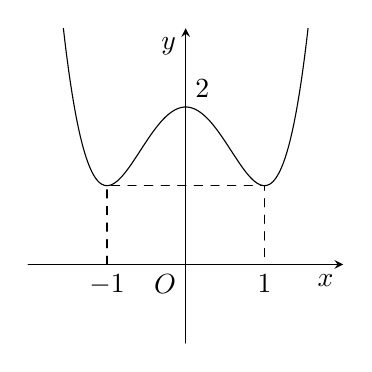
\begin{tikzpicture}[line cap=round,>=stealth,scale=1]
					%		\tikzset{every node/.style={scale=0.8}}
					\draw[->] (-2,0)--(2,0) node[below left] {$x$};
					\draw[->] (0,-1)--(0,3) node[below left] {$y$};
					\draw (0,0) node [below left] {$O$};
					\draw[dashed,thin](-1,0) node[below] {$-1$}--(-1,1)--(1,1)--(1,0) node[below]{$1$} (0,2) node[above right]{$2$};
					\begin{scope}
						\clip (-2,-1) rectangle (2,3);
						\draw[samples=100,domain=-2:2,smooth,variable=\x] plot (\x,{abs(-1*((\x)^4)+2*((\x)^2)-2)});
					\end{scope}
				\end{tikzpicture}	
			\end{center}
			Dựa vào đồ thị ta nhận thấy điểm cực đại của đồ thị hàm số là $(0,2)$.
		\end{itemchoice}
	}
\end{ex}
\Closesolutionfile{ans}
\indapan{3}{ans/ans-2-B1-De1-DS}
%-------------------------------------------
\Opensolutionfile{ans}[ans/ans-2-B1-De1-KQ]
\caukq
\begin{ex}%[Câu 17]%[2D1H2-1]
	Cho hàm số $y=4x^3+8x^2-3x+3$. Giá trị cực đại của hàm số bằng bao nhiêu?
	\shortans[0]{12}
	\loigiai{
		Tập xác định $\mathbb{R}$.\\
		$y'=12x^2+16x-3$.\\
		$y'=0 \Leftrightarrow x=- \dfrac{3}{2} \text{ hoặc } x=\dfrac{1}{6}$.\\
		Hàm số đạt cực đại tại $x=- \dfrac{3}{2}, y_{\text{CĐ}}=12$.
	}
\end{ex}

\begin{ex}%[Câu 18]%[2D1H2-1]
	Tìm điểm cực tiểu của hàm số $y=x^3-5x^2-8x+8$?
	\shortans[0]{4}
	\loigiai{
		Tập xác định $\mathbb{R}$.\\
		$y'=3x^2-10x-8$.\\
		$y'=0 \Leftrightarrow x=- \dfrac{2}{3} \text{ hoặc } x=4$.\\
		Hàm số đạt cực tiểu tại $x=4, y_{\text{CT}}=-40$.
	}
\end{ex}

\begin{ex}%[Câu 19]%[2D1V1-3]
	Cho hàm số $y=-x^3-mx^2+(4m+9)x+3$ với $m$ là tham số. Có bao nhiêu giá trị nguyên của $m$ để hàm số nghịch biến trên $(-\infty;+\infty)$?
	\shortans[0]{7}
	\loigiai{
		Tập xác định $\mathbb{R}$.\\
		$y'=-3x^2-2mx+4m+9$.\\
		Hàm số nghịch biến trên $(-\infty;+\infty)$ khi $\heva{&a<0 \\ &\Delta\leq 0}$\\
		$ \Leftrightarrow m^2+12m+27 \leq 0$\\
		$ \Leftrightarrow -9\le m \le -3$.\\
		Suy ra $m \in \{-9,-8,-7,-6,-5,-4,-3\}$ 
	}
\end{ex}

\begin{ex}%[Câu 20]%[2D1V1-3]
	Đồ thị hàm số $y=x^3-3x^2+2ax+b$ có điểm cực tiểu $A(2;-2)$. Khi đó $a+b$ bằng bao nhiêu?
	\shortans[0]{2}
	\loigiai{
		$y'=3x^2-6x+2a$.\\
		Ta có hệ phương trình
		$\heva{&4a+b=2 \\ &a=0} \Rightarrow \heva{&a=0 \\ &b=2.}$\\
		Vậy $a+b=2$.
	}
\end{ex}

\begin{ex}%[Câu 21]%[2D1C1-3]
	Có bao nhiêu giá trị nguyên của tham số $m$ để hàm số $y=x^3-3(m+2)x^2+3(m^2+4m)x+1$ nghịch biến trên khoảng $(0; 1)$?
	\shortans[0]{4}
	\loigiai{
		Hàm số nghịch biến trên $(0; 1)$ khi và chỉ khi
		\begin{eqnarray*}
			y'\leq 0,\quad \forall x\in (0; 1)&\Leftrightarrow& 3x^2-6(m+2)x+3(m^2+4m)\leq 0,\quad \forall x\in (0; 1)\\
			&\Leftrightarrow&(x-m)(3x-3m-12)\leq 0,\quad \forall x\in (0; 1)\\
			&\Leftrightarrow& m\leq x\leq m+4,\quad \forall x\in (0; 1)\\
			&\Leftrightarrow&\heva{&m\leq 0\\&1\leq m+4}\Leftrightarrow -3\leq m\leq 0.
		\end{eqnarray*}
		Suy ra có $4$ giá trị của $m$ thỏa mãn đề bài.
	}
\end{ex}

\begin{ex}%[Câu 22]%[2D1C1-3]
	Tìm giá trị của tham số $m$ để ba điểm cực trị của đồ thị hàm số $y=x^4+(6m-4)x^2+1-m$ là ba đỉnh của một tam giác vuông? (Kết quả làm tròn đến chữ số hàng phần trăm).
	\shortans[0]{0,33}
	\loigiai{
		Ta có $y'=4x^3+4(3m-2)x.$ Giải $y'=0\Leftrightarrow \hoac{&x=0\\&x^2=2-3m.}$\\
		Hàm số có ba cực trị khi và chỉ khi $y'=0$ có ba nghiệm phân biệt $\Leftrightarrow 2-3m>0\Leftrightarrow m<\dfrac{2}{3}.$\\
		Khi đó, tọa độ ba điểm cực trị là $A(0;10m),$ $B\left(\sqrt{2-3m};-(2-3m)^2+1-m\right)$ \\
		và $C\left(-\sqrt{2-3m};-(2-3m)^2+1-m\right).$\\
		Ta có $\overrightarrow{AB}=\left(\sqrt{2-3m};-(2-3m)^2\right)$ và $\overrightarrow{AC}=\left(-\sqrt{2-3m};-(2-3m)^2\right)$ \\
		Nhận xét: $\triangle ABC$ luôn cân tại $A.$\\
		Do đó $A$, $B$, $C$ tạo thành tam giác vuông $\Leftrightarrow \overrightarrow{AB} \cdot \overrightarrow{AC}=0\Leftrightarrow -(2-3m)+(2-3m)^4=0$\\
		$\Leftrightarrow (2-3m)^3=1\Leftrightarrow m=\dfrac{1}{3}.$ 
	}
\end{ex}
\Closesolutionfile{ans}
\indapan{6}{ans/ans-2-B1-De1-KQ}